\subsection{问题二：催化剂组合与温度的影响分析}

本问需要区分温度和催化剂组合各自对应的变化。为判断温度影响，比较同一组合升温前后
的指标；为判断组合影响，比较同一温度下的不同组合。在此基础上，再检查不同组合的
升温幅度是否一致，并通过删去一种组合或一个温度考察结论是否依赖特定数据。

\subsubsection{共同温度上的可比数据}

附件 1 中，21 种催化剂组合在 250、275、300 和 350~℃下都有记录。本文以这 84 条
记录作为主体数据：比较温度时始终使用相同的 21 种组合，比较组合时始终使用相同的
4 个温度，从而避免把比较对象改变造成的差别混入因素影响。
325~℃和400~℃只在拥有相邻记录的相同组合中作补充配对；450~℃仅有A3的一条记录，
不参与跨组合归纳。

\subsubsection{温度影响：同一组合升温前后的变化}

设 \(Z_i(T_j)\) 表示组合 \(i\) 在温度 \(T_j\) 下的转化率或 C4 烯烃选择性。对同一
组合的相邻共同温度记录作差：

\begin{equation}
\Delta Z_{ij}=Z_i(T_{j+1})-Z_i(T_j).
\tag{15}
\label{eq:q2-paired-change}
\end{equation}

\(\Delta Z_{ij}>0\) 表示该组合在较高温度下指标更高；小于或等于 0 的记录作为局部
例外保留。该差值只比较真实观测，不假定连续温度函数。

表\ref{tab:q2-paired-change}汇总21种组合在三个共同温区内的配对变化。
\begin{table}[H]
\centering
\caption{相同21种组合在相邻共同温度间的配对变化}
\label{tab:q2-paired-change}
\begin{tabular}{lrrrr}
\toprule
温区 & 转化率正向数 & 转化率中位变化 & 选择性正向数 & 选择性中位变化 \\
 & （个） & （百分点） & （个） & （百分点） \\
\midrule
250--275~℃ & 19 & 2.010 & 17，另有1个持平 & 1.930 \\
275--300~℃ & 21 & 3.800 & 20 & 3.110 \\
300--350~℃ & 21 & 13.880 & 21 & 10.720 \\
\bottomrule
\end{tabular}
\end{table}

表中可见，275--350~℃内两个指标几乎都随温度升高而增加，
且300--350~℃的中位增量最大；250--275~℃仍有少数下降或持平。因此，温度升高通常
对应更高的转化率和选择性，但不能表述成每种组合在每个温区都严格增加。325~℃和
400~℃的匹配补充比较也得到正的中位变化，与主体方向一致。

\subsubsection{组合影响：同温比较与扣除温度差异}

在每个共同温度内，将21种组合按指标值由高到低排序，再比较四个温度的平均名次。
转化率平均名次前五为A7、A2、A3、A6和A5；C4 烯烃选择性平均名次前五为A1、A2、
A9、A4和A3。A2和A3在两个指标中都处于前列，A7主要表现为转化率较高，A1主要表现
为选择性较高。因此，“较好的组合”必须说明评价的是哪个指标。

上述排名直接比较同温表现。为了进一步给出可量化的组合差异，将每个观测值拆成
``总体水平、组合偏差、温度偏差和剩余变化''四部分。记 \(y_{ij}\) 为组合 \(i\) 在
温度 \(j\) 下的观测值，则

\begin{equation}
y_{ij}=\mu+\alpha_i+\beta_j+r_{ij}.
\tag{16}
\label{eq:q2-additive}
\end{equation}

其中，\(\mu\) 是 84 个观测的总体均值；\(\alpha_i\) 表示组合 \(i\) 在四个温度下
平均比总体水平高或低多少；\(\beta_j\) 表示温度 \(j\) 下的总体升降；\(r_{ij}\) 是
前三部分相加后仍不能解释的差值。取
\(\sum_i\alpha_i=0\) 和 \(\sum_j\beta_j=0\)，则

\begin{align}
\alpha_i&=\bar y_{i\cdot}-\bar y_{\cdot\cdot},&
\beta_j&=\bar y_{\cdot j}-\bar y_{\cdot\cdot}, \tag{17}\label{eq:q2-effects}\\
r_{ij}&=y_{ij}-\bar y_{i\cdot}-\bar y_{\cdot j}+\bar y_{\cdot\cdot}.
\tag{18}\label{eq:q2-residual}
\end{align}

图\ref{fig:q2-combination-effect}比较扣除温度总体差异后的组合偏差。
\begin{figure}[H]
\centering
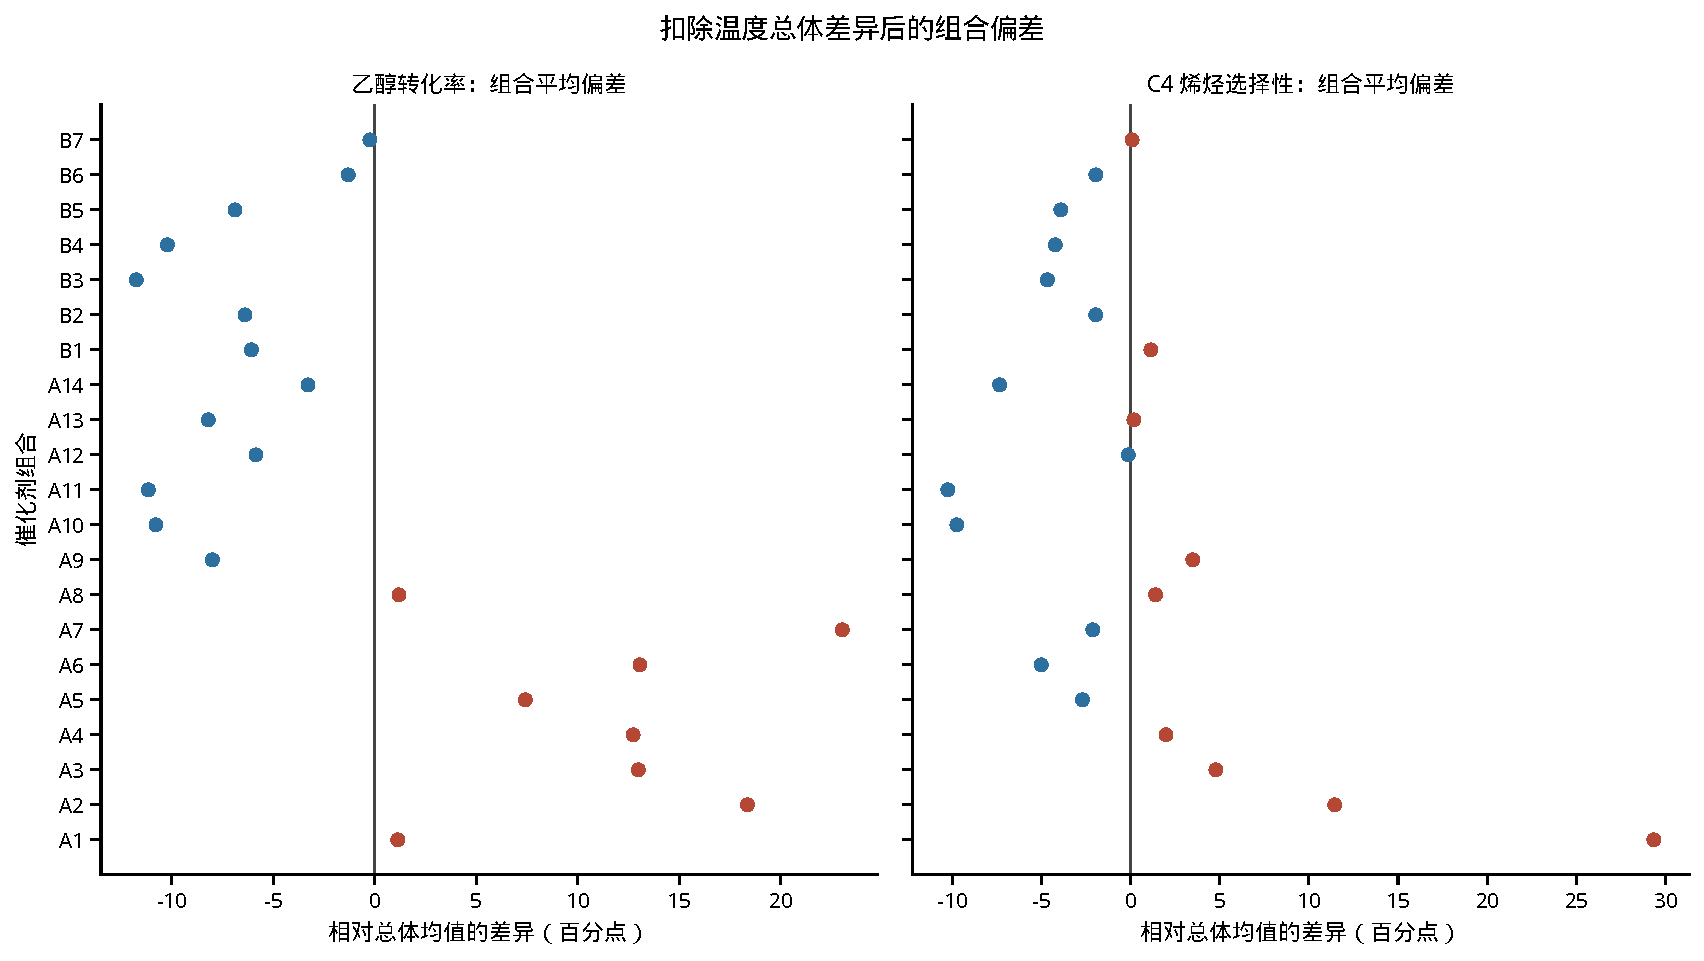
\includegraphics[width=0.94\linewidth]{../../output/q2/figures/01_additive_combination_effects.pdf}
\caption{扣除温度总体差异后的催化剂组合偏差。正值表示该组合跨四个共同温度的平均值
高于总体均值，负值表示低于总体均值。}
\label{fig:q2-combination-effect}
\end{figure}

图中转化率偏差最高的A7比
总体均值高23.043个百分点，最低的B3低11.737个百分点；选择性偏差最高的A1高
29.347个百分点，最低的A11低10.243个百分点。该高低格局与同温排名一致；在扣除
四个温度各自的总体均值差异后，组合之间仍保留数值差别。

\subsubsection{组合与温度的非加和变化}

如果所有组合升温时都增加相同的幅度，那么总体水平、组合偏差和温度偏差三项就足以
还原观测值。式\eqref{eq:q2-residual}中的 \(r_{ij}\) 正是实际值与这一简单还原值的
差；绝对值越大，说明该组合在这个温度下的变化越特殊。由于每个组合—温度条件只有
一次观测，该差值还包含实验误差和未记录因素，不能认定为只由组合与温度共同作用
产生的独立部分。

图\ref{fig:q2-residual}给出每个组合—温度单元未被简单加和结构解释的差值。
\begin{figure}[H]
\centering
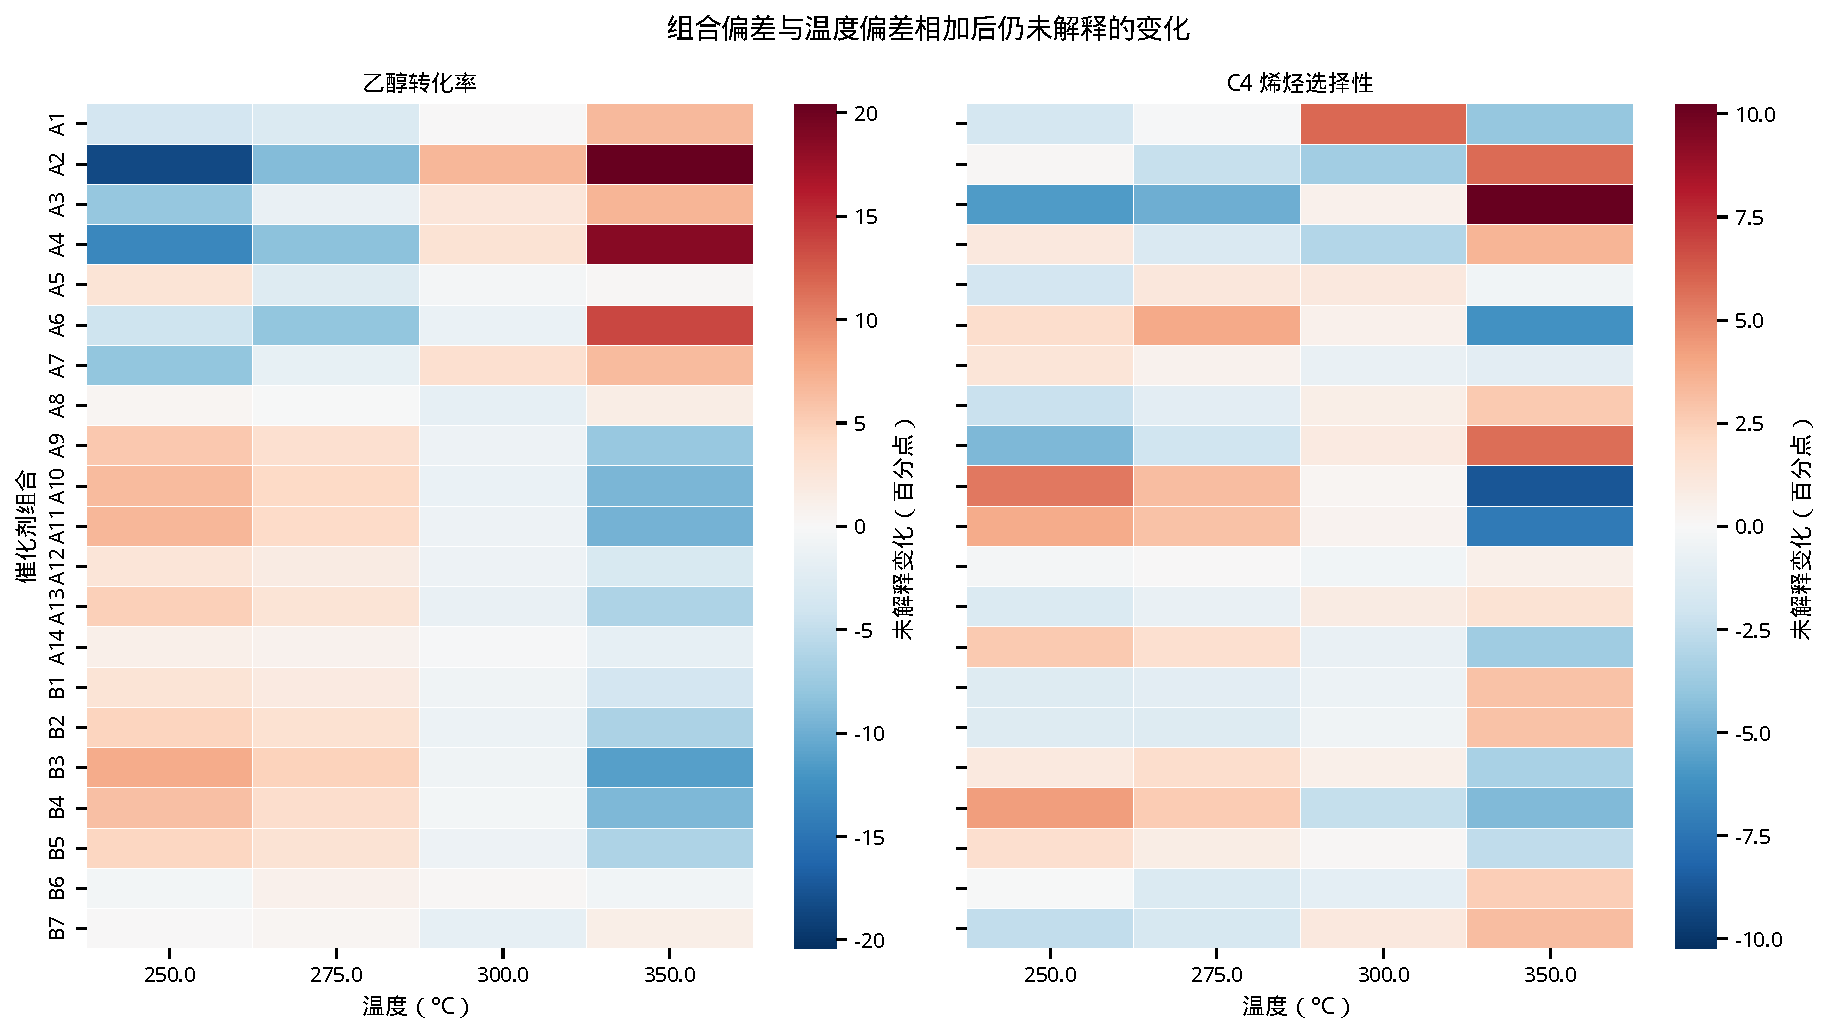
\includegraphics[width=0.90\linewidth]{../../output/q2/figures/03_nonadditive_residual_heatmaps.pdf}
\caption{组合偏差与温度偏差简单相加后仍未解释的单元变化。颜色深浅表示偏离大小，
正负号表示实际值高于或低于加和概括值。}
\label{fig:q2-residual}
\end{figure}

图中转化率偏离最大的单元为A2在350~℃，实际值比加和概括值
高20.441个百分点；选择性偏离最大的单元为A3在350~℃，高10.244个百分点。这说明
不同组合虽然大多随温度上升，但升高幅度并不一致，即组合与温度存在非加和变化迹象。

为比较三类差异的总体大小，分别计算组合偏差、温度偏差和剩余变化的平方和，再除以
84 个观测的总离差平方和。所得比例之和为 1，表示当前数据的差异主要出现在哪一部分，
不表示三个因素各自造成了多少结果。

表\ref{tab:q2-decomposition}比较三类差异在主体数据总离差中的比例。
\begin{table}[H]
\centering
\caption{三类差异占主体数据总差异的比例}
\label{tab:q2-decomposition}
\begin{tabular}{lrrr}
\toprule
考察指标 & 组合间差异 & 温度间差异 & 未解释变化 \\
\midrule
乙醇转化率 & 45.61\% & 38.40\% & 15.99\% \\
C4 烯烃选择性 & 59.69\% & 31.82\% & 8.48\% \\
\bottomrule
\end{tabular}
\end{table}

在当前21种组合和四个共同温度内，两个指标的组合间差异均大于温度间差异；但这一
大小次序是否稳定，还需通过改变组合集合和温度范围检查。

\subsubsection{删除组合或温度后的范围检查}

为检查结论是否依赖某一种组合或某一个温度，两个响应分别进行21次整组删除和4次
整温度删除，共 \(2\times(21+4)=50\) 次结构保持型重新计算。整组删除后每次保留
\(20\times4=80\) 个单元，删除温度后每次保留 \(21\times3=63\) 个单元；这里的50
表示模型复算次数，不是新增实验数或被删除的数据条数。所有删减情形下，两个指标的
跨组合均值仍随温度严格增加；原来排名前五和后五
的组合至少有 80\% 仍留在相应集合中。因此，温度影响的总体方向和主要的高低组合不由
某一个组合或温度单独决定。

但是，``组合间差异大于温度间差异''会随比较范围改变。删除A7后，转化率的组合比例
40.53\%低于温度比例41.24\%；删除A1后，选择性的组合比例34.84\%低于温度比例
51.95\%；删除300~℃后，转化率也出现次序反转。A7和A1分别是对应指标中组合偏差
最大的组合，删除它们会缩小组合间差异；删除一个温度则改变温度范围。所以
表\ref{tab:q2-decomposition}只说明当前 21 种组合和四个温度中的相对大小。

\subsubsection{问题二结论与适用范围}

已有研究表明，乙醇形成较高碳数产物可能经历乙醛生成、缩合、氢转移和脱水等连续步骤，
不同产物路径之间也会相互竞争 \cite{ho2016,moteki2016}。不同催化剂组合可能使这些
步骤对温度的响应不同，从而出现不同的升温幅度。这是与数据相容的一种解释，但文献中
的催化体系与本题并不相同，现有数据也不足以判断具体反应路径或某一种配方成分的作用。

综上，温度影响由同一组合的配对变化回答：升温通常对应更高的转化率和选择性，但
低温段存在少数例外。组合影响由同温排名和扣除温度差异后的组合偏差回答：不同组合
的观测表现存在差异，且两个指标的优势组合不完全相同。非加和剩余进一步表明，不同组合
的升温幅度并不一致。前两项结论较稳定，三类差异的相对大小则依赖纳入的组合和温度
范围；以上关系均限于已测对象和温度，不能作为化学因果作用或未测条件预测。
